% Compilar com XeLaTeX (no Overleaf: Menu > Compiler > XeLaTeX)
\documentclass[aspectratio=169,10pt,xcolor=table]{beamer}
\usetheme[progressbar=frametitle, numbering=fraction]{metropolis}
\usepackage{babel}
\babelprovide[import, main]{portuguese}
\usepackage{amsmath, amssymb}
\usepackage{booktabs, array, tabularx}
\usepackage{tikz}
\usetikzlibrary{arrows.meta, positioning}
\usepackage{pgfplots}
\pgfplotsset{compat=1.17}

% ---------- cores
\definecolor{mar}{HTML}{0B2A3C}
\definecolor{marmedio}{HTML}{0B3D5C}
\definecolor{teal}{HTML}{0E7C86}
\definecolor{laranja}{HTML}{F28C38}
\definecolor{cinza}{HTML}{A9BCC6}
\definecolor{azul}{HTML}{5FA8D3}
\definecolor{nevoa}{HTML}{EAF2F6}
\definecolor{areia}{HTML}{FDEBDB}
\definecolor{texto2}{HTML}{4A6573}
\definecolor{coral}{HTML}{C8553D}
\setbeamercolor{normal text}{fg=mar}
\setbeamercolor{frametitle}{bg=marmedio, fg=white}
\setbeamercolor{progress bar}{fg=laranja, bg=nevoa}
\setbeamercolor{title separator}{fg=laranja}
\setbeamercolor{alerted text}{fg=laranja}
\setbeamercolor{example text}{fg=teal}
\setbeamercolor{block title}{bg=nevoa, fg=teal}
\setbeamercolor{block body}{bg=nevoa!60}
\setbeamercolor{block title alerted}{bg=areia, fg=laranja}
\setbeamercolor{block body alerted}{bg=areia!60}
\setbeamertemplate{blocks}[rounded]

% ---------- atalhos
\newcommand{\cartao}[3][nevoa]{%
  \begin{tcolorbox}[colback=#1, colframe=#1]
  {\color{teal}\bfseries #2}\par\smallskip #3
  \end{tcolorbox}}
\usepackage[most]{tcolorbox}
\tcbset{arc=2mm, boxrule=0pt, left=2.5mm, right=2.5mm, top=1.5mm, bottom=1.5mm, before skip=1.5mm, after skip=1.5mm}
\newcommand{\cheio}{\tikz[baseline=-0.6ex]\fill[teal] (0,0) circle (1.1mm);}
\newcommand{\cheiol}{\tikz[baseline=-0.6ex]\fill[laranja] (0,0) circle (1.1mm);}
\newcommand{\vazio}{\tikz[baseline=-0.6ex]\draw[cinza] (0,0) circle (1.1mm);}
\newcommand{\grande}[2][laranja]{{\color{#1}\fontsize{24}{26}\selectfont\bfseries #2}}

\titlegraphic{\begin{tikzpicture}[remember picture, overlay, shift={(current page.south east)}, scale=0.75]
% fundo
\fill[nevoa] (-8,0) -- (-8,0.9) .. controls (-6.5,1.3) and (-5.5,0.6) .. (-4,1.0) .. controls (-2.5,1.4) and (-1.5,0.8) .. (0,1.1) -- (0,0) -- cycle;
% onda principal com tubo
\fill[teal] (-7.2,0) .. controls (-5.6,0.4) and (-4.6,1.6) .. (-3.9,3.0)
  .. controls (-3.5,3.8) and (-2.4,4.1) .. (-1.7,3.6)
  .. controls (-1.2,3.2) and (-1.4,2.5) .. (-1.9,2.4)
  .. controls (-2.3,2.35) and (-2.5,2.7) .. (-2.3,2.95)
  .. controls (-2.7,2.9) and (-2.9,2.4) .. (-2.6,2.0)
  .. controls (-2.0,1.3) and (-1.0,0.7) .. (0,0.6) -- (0,0) -- cycle;
% face interna (tubo)
\fill[marmedio] (-2.6,2.0) .. controls (-2.9,2.4) and (-2.7,2.9) .. (-2.3,2.95)
  .. controls (-2.5,2.7) and (-2.3,2.35) .. (-1.9,2.4)
  .. controls (-2.2,2.0) and (-2.0,1.5) .. (-1.2,1.0) .. controls (-1.7,1.2) and (-2.3,1.6) .. cycle;
% espuma da crista
\draw[white, line width=1.2pt, line cap=round] (-3.7,3.25) .. controls (-3.3,3.85) and (-2.4,4.0) .. (-1.85,3.6);
% frente
\fill[azul] (-8,0) -- (-8,0.55) .. controls (-6.8,0.85) and (-5.8,0.35) .. (-4.6,0.6) .. controls (-3.2,0.9) and (-1.8,0.3) .. (0,0.5) -- (0,0) -- cycle;

\end{tikzpicture}}
\title{Seleção ótima de ondas em uma sessão de surfe}
\subtitle{Em quais ondas remar para passar mais tempo em pé?}
\author{Luiz Felipe Píccoli Cavalini}
\institute{Otimização (COS360) · Escola Politécnica, UFRJ}
\date{}

\newcommand{\limi}[1]{\textcolor{laranja}{\textbullet}~\textcolor{white}{#1}\par\smallskip}
\begin{document}

\maketitle
\note{Bom dia. Meu trabalho trata a escolha de ondas numa sessão de surfe como um problema de otimização: em quais ondas remar para passar o maior tempo possível em pé.}

% ==================================================================
\begin{frame}{Motivação}
\begin{columns}[T]
\begin{column}{0.6\textwidth}
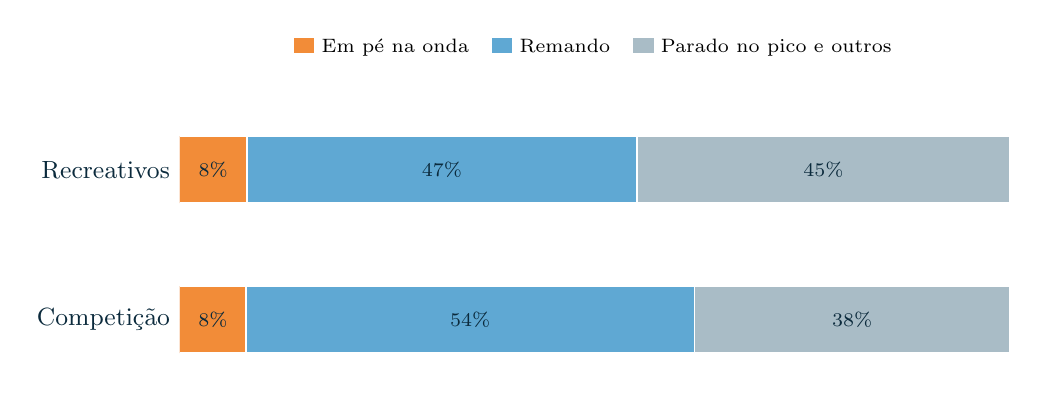
\begin{tikzpicture}
\begin{axis}[
  xbar stacked, width=\linewidth, height=5.2cm, bar width=0.85cm,
  xmin=0, xmax=100, axis x line=none, axis y line*=left, y axis line style={draw=none},
  symbolic y coords={Competição, Recreativos}, ytick=data, enlarge y limits=0.45,
  yticklabel style={font=\small, color=mar},
  nodes near coords={\pgfmathprintnumber[fixed, precision=0]{\pgfplotspointmeta}\%}, nodes near coords style={font=\scriptsize, color=mar},
  legend style={at={(0.5,1.12)}, anchor=south, legend columns=-1, draw=none, font=\scriptsize, /tikz/every even column/.append style={column sep=2mm}},
  reverse legend=false, every axis plot/.append style={draw=white, line width=0.6pt}]
\addplot[fill=laranja] coordinates {(8,Competição) (8.1,Recreativos)};
\addplot[fill=azul] coordinates {(54,Competição) (47,Recreativos)};
\addplot[fill=cinza] coordinates {(38,Competição) (44.9,Recreativos)};
\legend{Em pé na onda, Remando, Parado no pico e outros}
\end{axis}
\end{tikzpicture}
\end{column}
\begin{column}{0.37\textwidth}
\begin{tcolorbox}[colback=areia, colframe=areia, arc=2mm]
\grande{8\%}\par
do tempo é passado em pé na onda
\end{tcolorbox}
{\scriptsize\color{texto2}
\textbf{Recreativos:} 60 sessões de 39 surfistas, GPS (Barlow et al., 2014).\par\smallskip
\textbf{Competição:} Farley et al. (2012); cinza = 100\% menos remando e em pé.\par}
\medskip
{\footnotesize\color{teal}\bfseries Pergunta: em quais ondas remar para passar o máximo de tempo em pé?}
\end{column}
\end{columns}
\note{Estudos com GPS mostram que só cerca de 8\% de uma sessão é passada em pé na onda; quase metade do tempo é remando. Ou seja, o tempo em pé é escasso, e cada onda tem um custo. A pergunta do trabalho é: em quais ondas remar para passar o máximo de tempo em pé?}
\end{frame}

% ==================================================================
\begin{frame}{Por que a escolha das ondas é difícil?}
\begin{columns}[T]
\begin{column}{0.49\textwidth}
\cartao{Séries}{As ondas chegam em grupos de 3 a 5, separados por minutos de calmaria.}
\cartao{Ondas na cabeça}{Sem canal no pico, as ondas que chegam durante a volta atingem o surfista e o atrasam.}
\end{column}
\begin{column}{0.49\textwidth}
\cartao{Tempo ocupado}{Depois de surfar, é preciso remar de volta ao pico: cerca de 5\,s de remada (estimativa) para cada segundo em pé.}
\cartao{Fôlego}{Cada onda gasta energia; o surfista só recupera fôlego enquanto espera no pico.}
\end{column}
\end{columns}
\begin{tcolorbox}[colback=areia, colframe=areia, arc=2mm]
{\color{laranja}\bfseries Consequência:} pegar a maior onda de uma série pode fazer o surfista perder a série seguinte ou ficar sem fôlego para ela.
\end{tcolorbox}
\note{Quatro fatores complicam a escolha. As ondas chegam em séries, separadas por calmarias. Depois de surfar, é preciso remar de volta ao pico: cerca de cinco segundos de remada por segundo em pé. Sem canal, as ondas que chegam na volta atingem o surfista e o atrasam. E cada onda gasta fôlego, que só se recupera esperando no pico. Resultado: pegar a maior onda pode custar a série seguinte.}
\end{frame}

% ==================================================================
\begin{frame}{Exemplo ilustrativo}
\noindent\textcolor{teal}{\small\bfseries Fôlego máximo 200; recupera 1 unidade por segundo de espera no pico.}\par
\smallskip

\centering
\small
\renewcommand{\arraystretch}{1.25}
\setlength{\tabcolsep}{9pt}
\begin{tabular}{l *{3}{c} p{2pt} *{3}{c} c}
 & \multicolumn{3}{c}{\footnotesize\textcolor{texto2}{Série 1}} & & \multicolumn{3}{c}{\footnotesize\textcolor{texto2}{Série 2}} & \\
\textbf{Onda} & \textbf{1} & \textbf{2} & \textbf{3} & & \textbf{4} & \textbf{5} & \textbf{6} & \textbf{Total} \\
\textcolor{teal}{\textbf{Segundos em pé}} & \textcolor{teal}{\textbf{10}} & \textcolor{teal}{\textbf{20}} & \textcolor{teal}{\textbf{30}} & & \textcolor{teal}{\textbf{10}} & \textcolor{teal}{\textbf{30}} & \textcolor{teal}{\textbf{20}} & \\
\textcolor{texto2}{Energia (custo)} & 95 & 120 & 200 & & 95 & 170 & 120 & \\
\midrule
\textbf{Gulosa} {\scriptsize\textcolor{texto2}{(pega o que der)}} & \cheio & \vazio & \vazio & & \cheio & \vazio & \vazio & \textbf{20\,s} \\
\textbf{Paciente} {\scriptsize\textcolor{texto2}{(só a maior)}} & \vazio & \vazio & \cheio & & \vazio & \vazio & \vazio & \textbf{30\,s} \\
\rowcolor{areia}\textcolor{laranja}{\textbf{Ótimo}} {\scriptsize\textcolor{texto2}{(modelo)}} & \cheiol & \vazio & \vazio & & \vazio & \cheiol & \vazio & \textcolor{laranja}{\textbf{40\,s}} \\
\end{tabular}

\medskip
\begin{tcolorbox}[colback=nevoa, colframe=nevoa]
\footnotesize\textbf{Por que não as ondas 2 e 5 (50\,s)?} Depois da onda 2 restam 80; o surfista espera só 40\,s e chega à onda 5 com 120, menos que os 170 necessários. Com a onda 1, ele espera 90\,s e chega com 195.
\end{tcolorbox}
\note{Aqui há seis ondas em duas séries, com os segundos em pé e o custo de energia de cada uma. O fôlego máximo é 200 e recupera 1 por segundo de espera. A regra gulosa, que pega toda onda possível, faz 20 segundos. A regra paciente pega a maior onda, a 3, gasta todo o fôlego e perde a série 2: 30 segundos. O ótimo pega a onda 1, descansa 90 segundos e chega à onda 5 com fôlego: 40 segundos. As ondas 2 e 5 dariam 50, mas o surfista chegaria à onda 5 com 120 de energia, menos que os 170 necessários.}
\end{frame}

% ==================================================================
\begin{frame}{Modelo matemático (1/2): grafo, dados e variáveis}
\begin{columns}[T]
\begin{column}{0.5\textwidth}
\centering
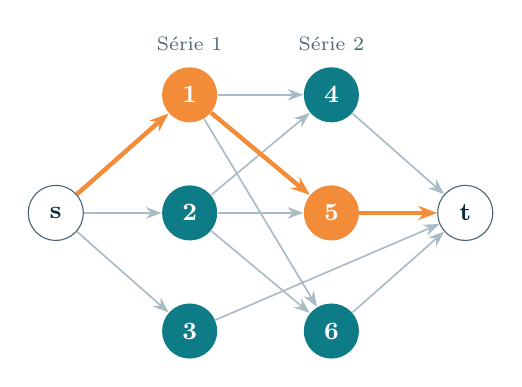
\begin{tikzpicture}[
  no/.style={circle, minimum size=7mm, inner sep=0, font=\small\bfseries},
  onda/.style={no, fill=teal, text=white},
  otimo/.style={no, fill=laranja, text=white},
  ext/.style={no, draw=texto2, fill=white, text=mar},
  arco/.style={-{Stealth[length=2mm]}, cinza, line width=0.6pt},
  arcoo/.style={-{Stealth[length=2.4mm]}, laranja, line width=1.6pt}]
\node[ext] (s) at (0,0) {s};
\node[otimo] (1) at (1.7,1.5) {1};
\node[onda] (2) at (1.7,0) {2};
\node[onda] (3) at (1.7,-1.5) {3};
\node[onda] (4) at (3.5,1.5) {4};
\node[otimo] (5) at (3.5,0) {5};
\node[onda] (6) at (3.5,-1.5) {6};
\node[ext] (t) at (5.2,0) {t};
\node[font=\scriptsize, color=texto2] at (1.7,2.15) {Série 1};
\node[font=\scriptsize, color=texto2] at (3.5,2.15) {Série 2};
\foreach \a/\b in {s/2, s/3, 1/4, 1/6, 2/4, 2/5, 2/6, 3/t, 4/t, 6/t} \draw[arco] (\a) -- (\b);
\foreach \a/\b in {s/1, 1/5, 5/t} \draw[arcoo] (\a) -- (\b);
\end{tikzpicture}

\medskip
{\scriptsize\color{texto2}\raggedright Cada onda é um nó. Só existe seta de $i$ para $j$ se dá tempo de voltar ao pico depois de $i$ antes de $j$ chegar: $a_i + d_i \le a_j$. Cada caminho de $s$ a $t$ é uma sessão possível.\par}
\end{column}
\begin{column}{0.47\textwidth}
{\color{teal}\bfseries Dados}
\begin{tcolorbox}[colback=nevoa, colframe=nevoa]
\footnotesize
\begin{tabular}{@{}l p{5.2cm}@{}}
$a_i,\ v_i$ & chegada e duração da onda $i$ (s em pé) \\
$d_i$ & tempo ocupado: surfar + remar de volta + ondas na cabeça \\
$e_i$ & energia gasta para pegar a onda $i$ \\
$U,\ r$ & fôlego máximo e recuperação por segundo de espera \\
\end{tabular}
\end{tcolorbox}

\medskip
{\color{teal}\bfseries Variáveis de decisão}
\begin{tcolorbox}[colback=nevoa, colframe=nevoa]
\footnotesize
$y_{ij} \in \{0,1\}$: 1 se, depois da onda $i$, a próxima onda pega é a $j$\par\medskip
$f_{ij} \ge 0$: energia com que o surfista chega à onda $j$ vindo da onda $i$
\end{tcolorbox}
\end{column}
\end{columns}
\note{O modelo é um grafo. Cada onda é um nó; $s$ é a entrada na água e $t$, a saída. Há seta de $i$ para $j$ só se, depois de surfar $i$ e voltar ao pico, ainda dá tempo de pegar $j$. Assim, cada caminho de $s$ a $t$ é uma sessão possível; em laranja, o ótimo do exemplo. São duas variáveis: $y_{ij}$, binária, indica se a próxima onda depois de $i$ é $j$; e $f_{ij}$, contínua, é a energia com que o surfista chega a $j$ vindo de $i$.}
\end{frame}

% ==================================================================
\begin{frame}{Modelo matemático (2/2): função objetivo e restrições}
\footnotesize
\renewcommand{\arraystretch}{1.45}
\begin{tabularx}{\textwidth}{@{}>{\raggedright\arraybackslash}m{2.7cm} >{$}m{5.9cm}<{$} >{\raggedright\arraybackslash}X@{}}
\multicolumn{3}{@{}l}{\color{laranja}\bfseries\small Função objetivo} \\
\textcolor{teal}{\textbf{Maximizar}} & \max \textstyle\sum_{(i,j)\in A} v_j\, y_{ij} & Somar os segundos em pé das ondas escolhidas. \\
\multicolumn{3}{@{}l}{\color{laranja}\bfseries\small Restrições} \\
\textcolor{teal}{\textbf{Caminho único}} & \textstyle\sum_j y_{sj} = 1,\quad \sum_i y_{ik} = \sum_j y_{kj}\ \ \forall k & Sai uma vez de $s$; em cada onda, o que entra é igual ao que sai. \\
\textcolor{teal}{\textbf{Energia só em setas usadas}} & f_{ij} \le U\, y_{ij} & Energia só passa por setas escolhidas, até o máximo $U$. \\
\textcolor{teal}{\textbf{Fôlego suficiente}} & u_i \ge e_i \textstyle\sum_h y_{hi} & A energia ao chegar paga o custo da onda. \\
\textcolor{teal}{\textbf{Balanço de energia}} & \textstyle\sum_j f_{ij} \le u_i - e_i \sum_h y_{hi} + \sum_j r\, w_{ij}\, y_{ij} & O que chegou, menos o gasto, mais o recuperado na espera. \\
\textcolor{teal}{\textbf{Domínio}} & y_{ij} \in \{0,1\},\quad f_{ij} \ge 0 & Escolhas binárias (integralidade); energia não negativa. \\
\end{tabularx}

\vfill
{\scriptsize\color{texto2}Definições: $u_i = U\,y_{si} + \sum_h f_{hi}$ é a energia ao chegar na onda $i$; $w_{ij} = a_j - (a_i + d_i)$ é o tempo de espera no pico.}
\note{O objetivo soma os segundos em pé das ondas escolhidas. A primeira restrição forma um caminho único: o que entra numa onda, sai. A segunda só deixa passar energia pelas setas escolhidas, até o máximo $U$. A terceira exige energia suficiente para pagar a onda. A quarta é um balanço, como um estoque: sai o que chegou, menos o gasto, mais o recuperado na espera. Por fim, $y$ é binária e $f$ é não negativa.}
\end{frame}

% ==================================================================
\begin{frame}{Classificação do problema, solver e algoritmo}
\begin{columns}[T]
\begin{column}{0.55\textwidth}
\footnotesize
\cartao{Classificação}{Programa linear inteiro misto (MILP): objetivo e restrições lineares, $y$ binárias, $f$ contínuas. Caminho de maior valor com restrição de recurso, problema NP-difícil.}
\cartao{Solver}{Gurobi, chamado pelo Python (\texttt{gurobipy}). Cada sessão de 40 ondas ($\approx$1.500 variáveis) é resolvida em menos de 1\,s.}
\cartao{Algoritmo}{Branch and bound: resolve a relaxação linear (simplex), escolhe uma variável fracionária, divide em $y=0$ e $y=1$ e descarta ramos que não superam a melhor solução. O Gurobi acrescenta planos de corte.}
\end{column}
\begin{column}{0.42\textwidth}
\textcolor{teal}{\small\bfseries Por que não basta programação linear?}\par\smallskip
{\footnotesize Se $y$ pudesse ser fracionário ($0 \le y \le 1$), o solver misturaria duas sessões do exemplo:\par\smallskip
{\renewcommand{\arraystretch}{1.3}\begin{tabular}{@{}l r@{}}
$\tfrac23$ da sessão $s \to 1 \to 5 \to t$ & $\tfrac23 \times 40 = 26{,}7$\,s \\
$\tfrac13$ da sessão $s \to 2 \to 5 \to t$ & $\tfrac13 \times 50 = 16{,}7$\,s \\
\end{tabular}}\par\smallskip
Sozinha, a sessão pela onda 2 não tem fôlego para a 5; misturada, usa a energia que sobra da outra.\par}
\smallskip
\begin{tcbraster}[raster columns=2, raster equal height, raster column skip=2mm]
\begin{tcolorbox}[colback=areia, colframe=areia, halign=center]
\grande{43,3\,s}\par{\scriptsize relaxação: não é real}
\end{tcolorbox}
\begin{tcolorbox}[colback=nevoa, colframe=nevoa, halign=center]
\grande[marmedio]{40\,s}\par{\scriptsize ótimo inteiro (1 e 5)}
\end{tcolorbox}
\end{tcbraster}
\textcolor{teal}{\footnotesize\bfseries Por isso $y$ precisa ser binária.}\par
\end{column}
\end{columns}
\note{É um programa linear inteiro misto, e NP-difícil: num caso particular, ele vira o problema da mochila. Usei o Gurobi pelo Python, e sessões de 40 ondas saem em menos de um segundo. O algoritmo é o branch and bound: resolve a relaxação linear, escolhe uma variável fracionária, divide em zero e um, e descarta os ramos que não superam a melhor solução. À direita, o motivo de não bastar programação linear: se $y$ pudesse ser fracionário, o solver misturaria dois terços da sessão pelas ondas 1 e 5 com um terço da sessão pelas ondas 2 e 5, que sozinha não tem fôlego, e chegaria a 43,3 segundos. Isso não é uma sessão real; o ótimo inteiro é 40. Por isso $y$ precisa ser binária.}
\end{frame}

% ==================================================================
\begin{frame}{Resultados: sessões de 40 ondas}
\begin{columns}[T]
\begin{column}{0.58\textwidth}
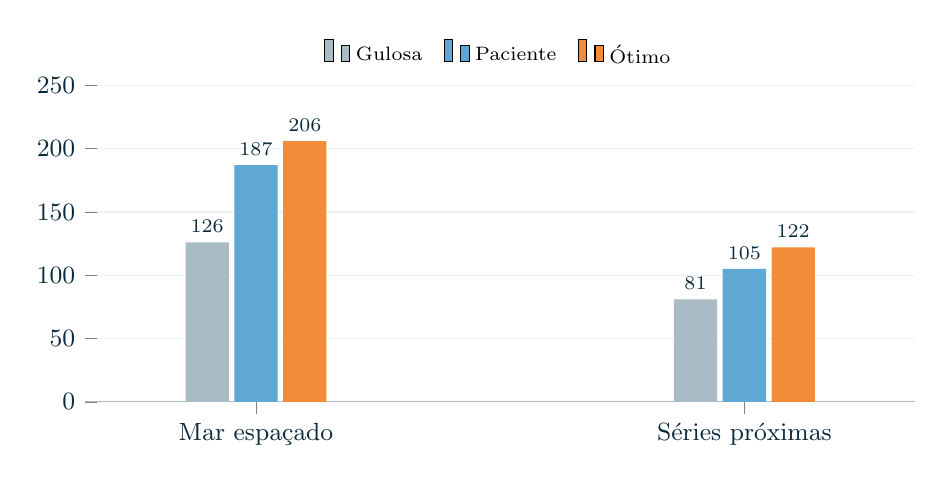
\begin{tikzpicture}
\begin{axis}[
  ybar, width=\linewidth, height=5.6cm, bar width=0.55cm,
  ymin=0, ymax=250, ytick={0,50,...,250}, ymajorgrids, grid style={color=nevoa},
  axis x line*=bottom, axis y line*=left, x axis line style={color=cinza}, y axis line style={draw=none},
  symbolic x coords={Mar espaçado, Séries próximas}, xtick=data, enlarge x limits=0.35,
  ticklabel style={font=\small, color=mar}, title={\small\color{texto2}Segundos em pé na sessão},
  nodes near coords, nodes near coords style={font=\scriptsize, color=mar},
  legend style={at={(0.5,1.02)}, anchor=south, legend columns=-1, draw=none, font=\scriptsize, /tikz/every even column/.append style={column sep=2mm}}]
\addplot[fill=cinza, draw=none] coordinates {(Mar espaçado,126) (Séries próximas,81)};
\addplot[fill=azul, draw=none] coordinates {(Mar espaçado,187) (Séries próximas,105)};
\addplot[fill=laranja, draw=none] coordinates {(Mar espaçado,206) (Séries próximas,122)};
\legend{Gulosa, Paciente, Ótimo}
\end{axis}
\end{tikzpicture}
\end{column}
\begin{column}{0.39\textwidth}
\begin{tcolorbox}[colback=areia, colframe=areia]
\grande{+16\%}\par{\small\bfseries séries próximas}\par{\scriptsize\color{texto2}122\,s contra 105\,s da regra paciente}
\end{tcolorbox}
\begin{tcolorbox}[colback=nevoa, colframe=nevoa]
\grande[marmedio]{+10\%}\par{\small\bfseries mar espaçado}\par{\scriptsize\color{texto2}206\,s contra 187\,s da regra paciente}
\end{tcolorbox}
{\footnotesize\color{teal}\bfseries O ótimo conhece todas as ondas; as regras não. A diferença é o ganho máximo possível, não o garantido.\par}
\smallskip
{\scriptsize\color{texto2}Mesmas 40 ondas sintéticas nos dois mares; só muda o intervalo entre as séries. Fôlego máximo 400, recuperação 0,5 por segundo.\par}
\end{column}
\end{columns}
\note{Em sessões sintéticas de 40 ondas, com fôlego 400 e recuperação 0,5, o ótimo faz 10\% a mais que a regra paciente no mar espaçado e 16\% a mais com séries próximas. Mas o modelo conhece todas as ondas de antemão, e as regras não. Por isso, esse é o ganho máximo possível, não um ganho garantido.}
\end{frame}

% ==================================================================
\begin{frame}{Conclusão}
\begin{columns}[T]
\begin{column}{0.58\textwidth}
\begin{enumerate}
\setlength{\itemsep}{6pt}
\item[\color{laranja}\textbf{1}] \textbf{O fôlego é o que torna o problema difícil.}\\
{\small\color{texto2}Com recuperação, o custo de cada onda depende de quanto o surfista descansou antes: programa inteiro misto.}
\item[\color{laranja}\textbf{2}] \textbf{As regras simples perdem tempo em pé.}\\
{\small\color{texto2}Neste cenário, o ótimo supera a regra paciente em 10\% a 16\%; a perda é maior com séries próximas.}
\item[\color{laranja}\textbf{3}] \textbf{A formulação importa.}\\
{\small\color{texto2}Com big-M, a relaxação vale 285\,s contra 207\,s, e o solver demora muito mais.}
\end{enumerate}
\end{column}
\begin{column}{0.38\textwidth}
\begin{tcolorbox}[colback=marmedio, colframe=marmedio, coltext=white]
{\color{laranja}\bfseries Limitações}\par\smallskip
\footnotesize\color{white}
\setbeamercolor{itemize item}{fg=laranja}
\limi{Ondas conhecidas de antemão: o ótimo é um limite superior.}
\limi{Um surfista só, sem disputa de ondas.}
\limi{Sessões sintéticas; parâmetros estimados.}
\limi{Recuperação linear e só na espera.}
\end{tcolorbox}
\end{column}
\end{columns}
\note{Concluindo: o fôlego é o que torna o problema difícil; o ótimo faz até 16\% a mais que a melhor regra simples; e a formulação importa para o desempenho do solver. As limitações são ondas conhecidas de antemão, um surfista só e parâmetros estimados. Obrigado.}
\end{frame}

% ==================================================================
\begin{frame}{Referências}
\scriptsize
\begin{itemize}
\setlength{\itemsep}{5pt}
\item BARLOW, M. J. et al. The effect of wave conditions and surfer ability on performance and the physiological response of recreational surfers. \emph{J. Strength Cond. Res.}, 28(10), 2946--2953, 2014.
\item FARLEY, O. R. L.; HARRIS, N. K.; KILDING, A. E. Physiological demands of competitive surfing. \emph{J. Strength Cond. Res.}, 26(7), 1887--1896, 2012.
\item HOFFMAN, A. J.; KRUSKAL, J. B. Integral boundary points of convex polyhedra. In: \emph{Linear Inequalities and Related Systems}. Princeton, 1956.
\item JOKSCH, H. C. The shortest route problem with constraints. \emph{J. Math. Anal. Appl.}, 14(2), 191--197, 1966.
\item IRNICH, S.; DESAULNIERS, G. Shortest path problems with resource constraints. In: \emph{Column Generation}. Springer, 2005, p. 33--65.
\item LAND, A. H.; DOIG, A. G. An automatic method of solving discrete programming problems. \emph{Econometrica}, 28(3), 497--520, 1960.
\end{itemize}
\note{(Não é preciso falar nada. Deixe este slide aberto durante as perguntas.)}
\end{frame}

\end{document}
